\documentclass[12pt]{article}
\setlength{\oddsidemargin}{0in}
\setlength{\evensidemargin}{0in}
\setlength{\textwidth}{6.5in}
\setlength{\parindent}{0in}
\setlength{\parskip}{\baselineskip}

\usepackage{amsmath,amsfonts,amssymb,graphicx,hyperref}

%\title{Review of Newtonian Mechanics}

\begin{document}

PHYS 374 Fall 2020\hfill Worksheet 3: Shortest Path on a Cylinder and a Sphere\\
\\
Name: \\
\\
Please submit as a PDF on Moodle. Include any calculations made using external tools.

\hrulefill
\\
\\
\noindent
\textbf{Part I: }Consider a cylinder of radius $R$. The relationship between quantities in \href{https://mathworld.wolfram.com/CylindricalCoordinates.html}{Cylindrical} and Cartesian coordinates is
\begin{equation}
\begin{split}
x&=\rho\cos\phi\\
y&=\rho\sin\phi\\
z&=z
\end{split}
\end{equation}
\begin{enumerate}
\item Find the infinitesimal path length, $dl$ in cylindrical coordinates noting that the radius $\rho$ is fixed for the surface of a cylinder.
\item Use calculus of variations to find the shortest path on a cylinder with radius $R$ between two arbitrary points $A$ and $B$.
\item What is the shortest path if the starting and ending heights ($z$) are identical?
\item Does your answer in part 2. reduce to the correct answer? Discuss.
\item What is the shortest path if the starting and ending angles ($\phi$) are identical?
\item Does the answer in part 2. reduce to the correct answer?
%\begin{figure}[h]
%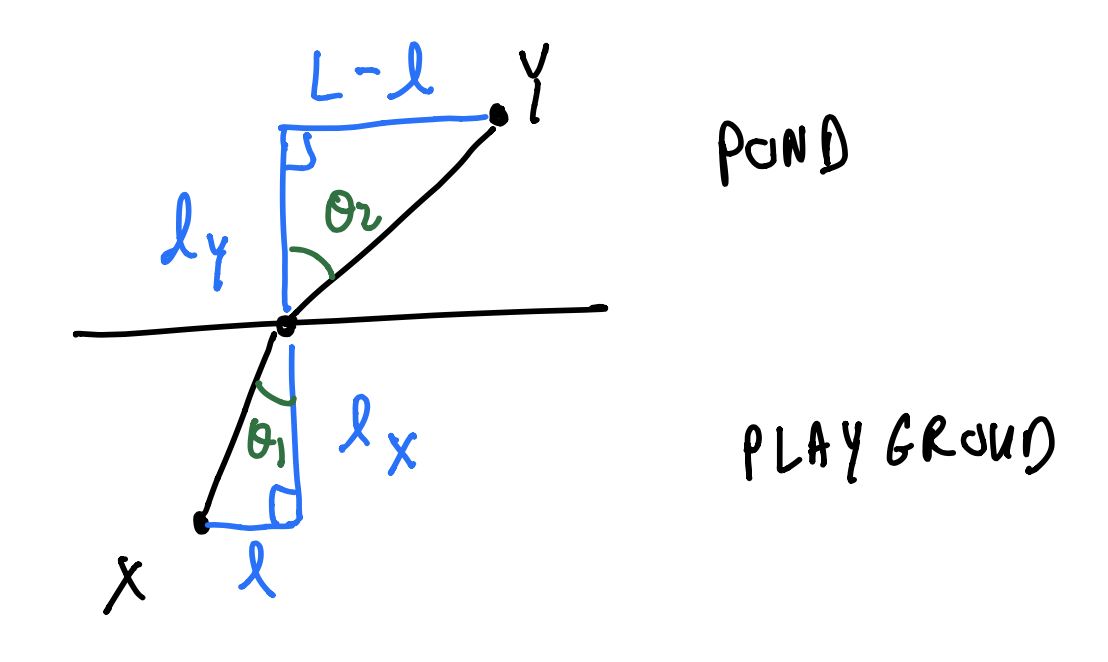
\includegraphics[width=8cm]{Diagram}
%\centering
%\end{figure}
\end{enumerate}
\textbf{Part II: }Consider a sphere of radius $R$. The relationship between quantities in \href{https://mathworld.wolfram.com/SphericalCoordinates.html}{Spherical} and Cartesian coordinates is
\begin{equation}
\begin{split}
x&=r\sin\theta\cos\phi\\
y&=r\sin\theta\sin\phi\\
z&=r\cos\theta
\end{split}
\end{equation}
\begin{enumerate}
\item Find the infinitesimal path length, $dl$ in spherical coordinates noting that the radius $r$ is fixed for the surface of a sphere.
\item Use calculus of variations to find the shortest path on a sphere with radius $R$ between two arbitrary points $A$ and $B$.
\item Discuss limiting cases.
\end{enumerate}
\end{document}